
\section{Classical ML model as Classifier}

    \begin{figure}
        \centering
        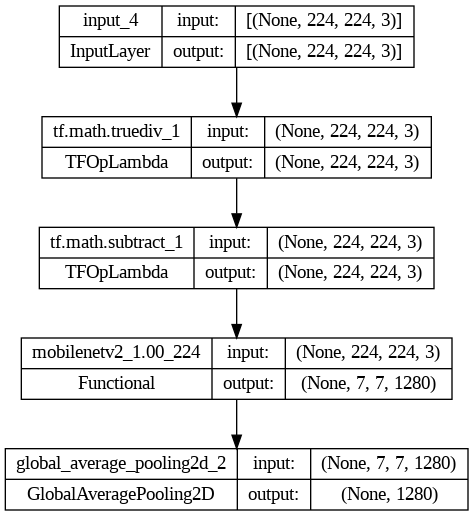
\includegraphics[width=0.75\linewidth]{graphics//chapter5/moboilenetv2 feature extractor.png}
        \caption{MobileNetV2 Feature Extractor used for training Classic ML Model}
        \label{fig:mobnetv2-feature-extractor}
    \end{figure}

\begin{figure}
    \centering
    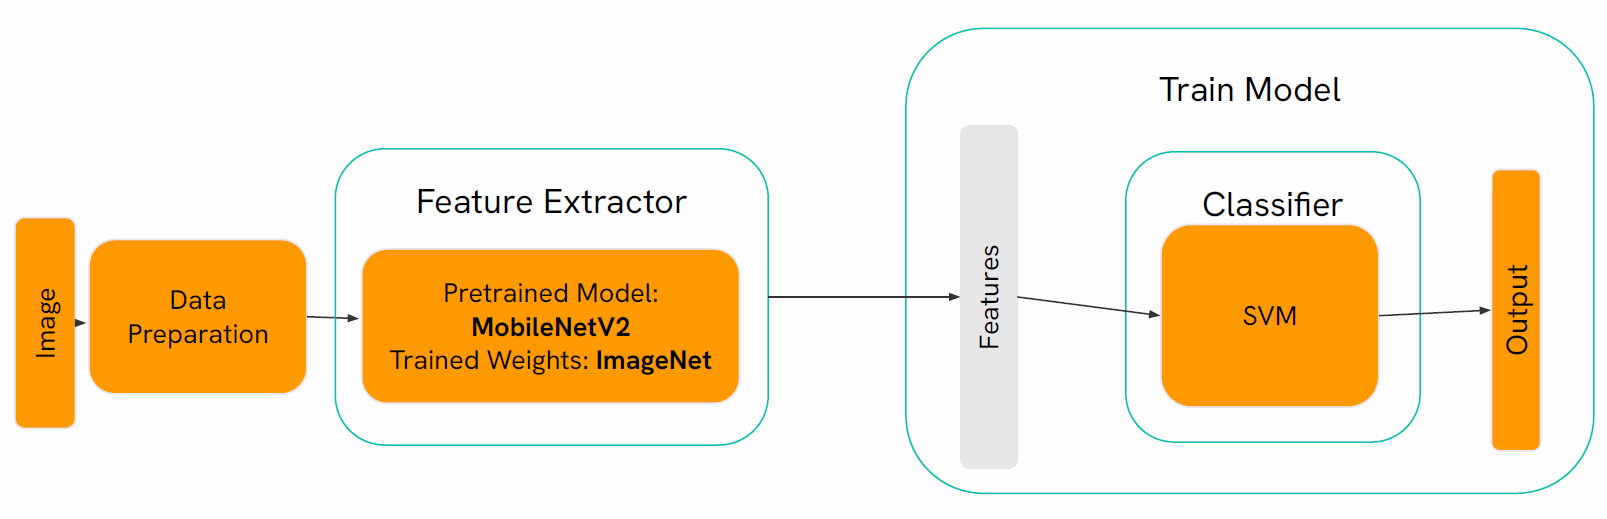
\includegraphics[width=1\linewidth]{graphics//chapter5/mobilenetV2 + SVM.png}
    \caption{MobilenetV2 + SVM}
    \label{fig:mobilenetv2-svm}
\end{figure}

\begin{figure}
    \centering
    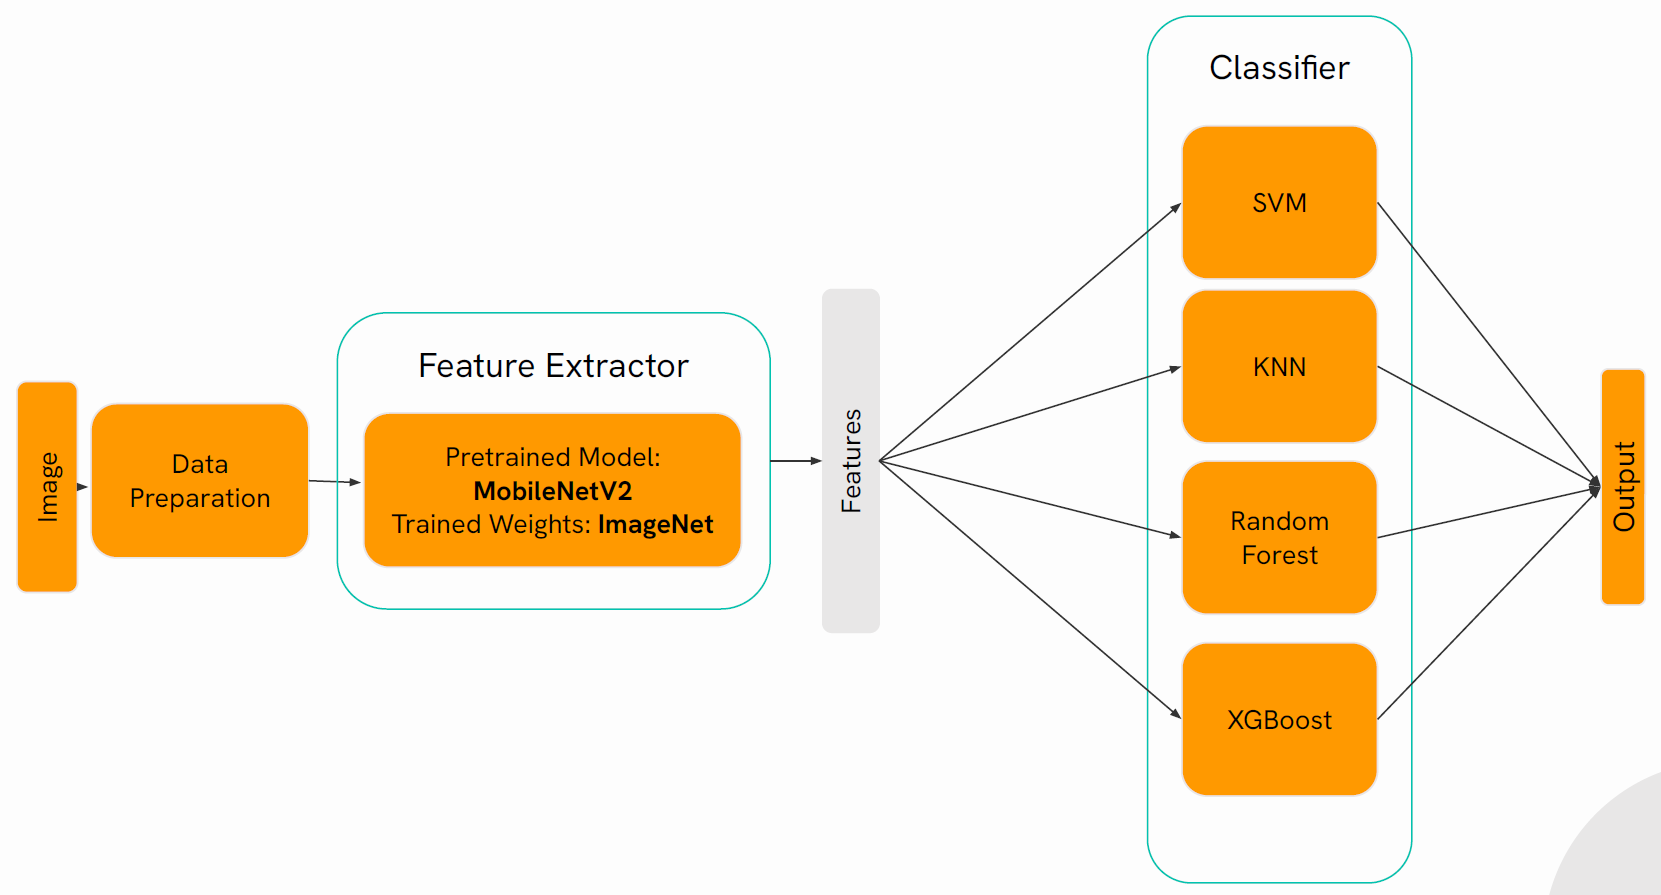
\includegraphics[width=1\linewidth]{graphics//chapter5/mobilentV2 + ML.png}
    \caption{MobileNetV2 + Traditional Classifier Models}
    \label{fig:mobilenetv2-all}
\end{figure}

    Since, classical ML classifier models such as SVM, KNN, Random forest, XBoost, etc cannot extract features directly from an image, we used a pretrained MobileNetV2 as a feature extractor for training these models.\par\vspace{1em}

    So, we first download a pretrained MobileNetV2 model (trained on \textbf{ImageNet}) and remove its top layer so that it gives the last feature maps as an output instead of the 1000 classes outputs. 
    Then, we input an image to this MobileNetV2, which give out a 7 x 7 x 1280 features map. we perform a global average pooling 2d on this output feature map to produce a 1280 features vector (7 x 7 x 1280 to 1 x 1 x 1280). \par\vspace{1em}
    In this way, we perform feature extraction for all the images in our dataset to convert it into 1280 feature vectors from an image of shape 256 x 256 x 3, then train our traditional classifier model on this extracted features
\FloatBarrier

